\documentclass[12pt]{article}

\usepackage[margin=1in]{geometry}
\usepackage{amsmath,amsthm,amssymb}
\usepackage{fancyhdr}
\usepackage[small,compact]{titlesec}
\usepackage{float}

\lhead{Erich Menge}
\chead{\classnameandsection}
\rhead{\homeworktitle}

\pagestyle{fancy}

\newcommand{\sethomeworknumber}[1]{
  \newcommand{\homeworktitle}{Homework #1}
}

\newcommand{\N}{\mathbb{N}}
\newcommand{\Z}{\mathbb{Z}}
\newcommand{\homeworkheader}[1]{
  \title{\vspace{2in}\homeworktitle}
  \author{Erich Menge (X.500: menge053, Student ID: 4624713) \\
  #1}
  \maketitle
  \newpage
}

\newenvironment{problem}[1]{
  \ignorespaces
  \section*{Problem #1}
}{
  \ignorespacesafterend
}

\newenvironment{solution}{
  \ignorespaces
  \subsection*{Solution}
}{
  \ignorespacesafterend
}

\newcommand{\classnameandsection}{CSCI 4011 Formal Languages And Automata Theory Section 3}

\usepackage{graphicx}
\usepackage{subfigure}

\sethomeworknumber{1}

\begin{document}
\homeworkheader{\classnameandsection}

\begin{problem}{1.6}

  Scrooge McNugget wants to store information (names, addresses, descriptions of embarrassing moments, etc.) about the
  many ducks on his payroll. Not surprisingly, the volume of data compels him to buy a database system. To save money,
  he wants to buy one with the fewest possible features, and he plans to run it as a stand-alone application on his PC
  clone. Of course, Scrooge does not plan to share his list with anyone. Indicate which of the following DBMS features
  Scrooge should pay for; in each case, also indicate why Scrooge should (or should not) pay for that feature in the
  system he buys.

  \begin{enumerate}
    \item A security facility.
    \item Concurrency control.
    \item Crash recovery.
    \item A view mechanism.
    \item A query language.
  \end{enumerate}

  \begin{solution}
    \begin{enumerate}
      \item Yes. He's putting it on his PC ``clone''. Because it is standalone and no one else needs to access it
      it should not accept network connections and should be located in a physically secure location. Physical access
      is total access.

      \item No. Since it is single-user there is no need for concurrency.

      \item Yes. Despite his frugality he is storing very valuable information (embarrassing moments) which he probably
      can't afford to lose. It would be good to make sure that in the event of a power outage his data isn't corrupted.

      \item Yes. While not strictly necessary, it may make Scrooge's life easier to create views. It doesn't specify
      if he will be using a program or accessing his database directly. If he is accessing it directly it may make sense
      for him to have views so that his work environment isn't as cluttered with less frequently used columns for instance.

      \item Yes. He will need to use the query language to interact with his database.
    \end{enumerate}
  \end{solution}
\end{problem}

\begin{problem}{2.2}

  A university database contains information about professors (identified by social security number, or SSN) and
  courses (identified by courseid). Professors teach courses; each of the following situations concerns the Teaches
  relationship set. For each situation, draw an ER diagram that describes it (assuming no further constraints hold).

  \begin{enumerate}
    \item Professors can teach the same course in several semesters, and each offering must be recorded.
    \item Professors can teach the same course in several semesters, and only the most recent such offering needs to be
      recorded. (Assume this condition applies in all subsequent questions.)
    \item Every professor must teach some course.
    \item Every professor teaches exactly one course (no more, no less).
    \item Every professor teaches exactly one course (no more, no less), and every course must be taught by some professor.
    \item Now suppose that certain courses can be taught by a team of professors jointly, but it is possible that no one
      professor in a team can teach the course. Model this situation, introducing additional entity sets and relationship
      sets if necessary.
  \end{enumerate}

  \begin{solution}
    \begin{figure}[H]
      \centering
      \caption{ER Diagrams}
      \subfigure[ER Diagram for 2.2-1]{
        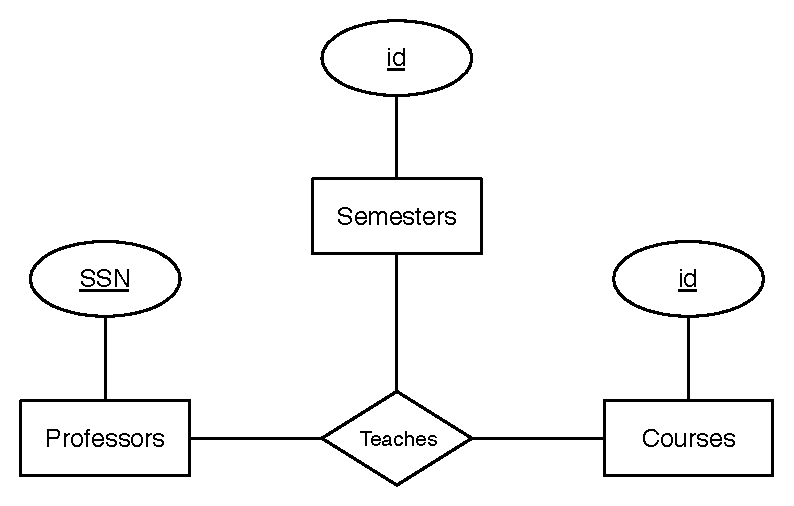
\includegraphics[scale=.5]{2_2_1.eps}
      } \qquad
      \subfigure[ER Diagram for 2.2-2]{
        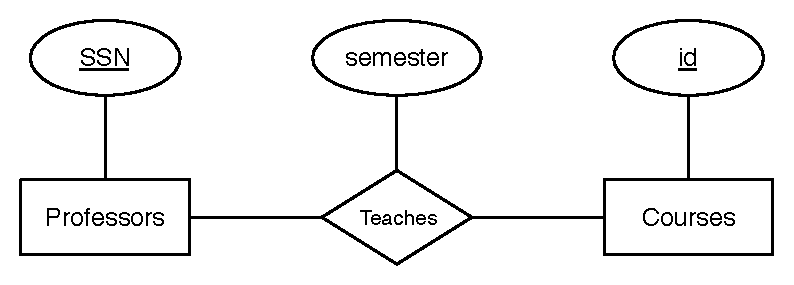
\includegraphics[scale=.5]{2_2_2.eps}
      } \qquad
      \subfigure[ER Diagram for 2.2-3]{
        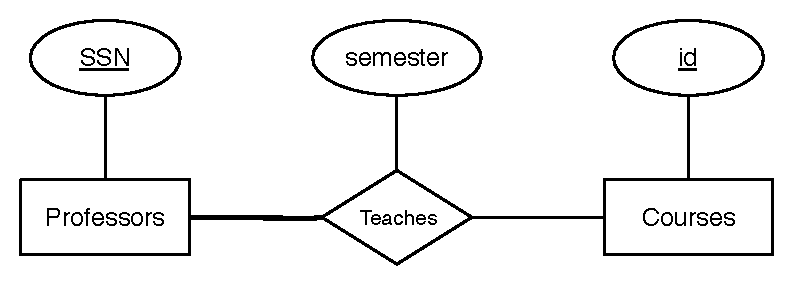
\includegraphics[scale=.5]{2_2_3.eps}
      } \qquad
      \subfigure[ER Diagram for 2.2-4]{
        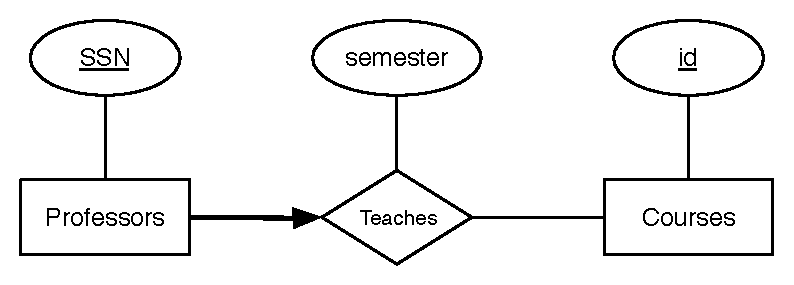
\includegraphics[scale=.5]{2_2_4.eps}
      } \qquad
      \subfigure[ER Diagram for 2.2-5]{
        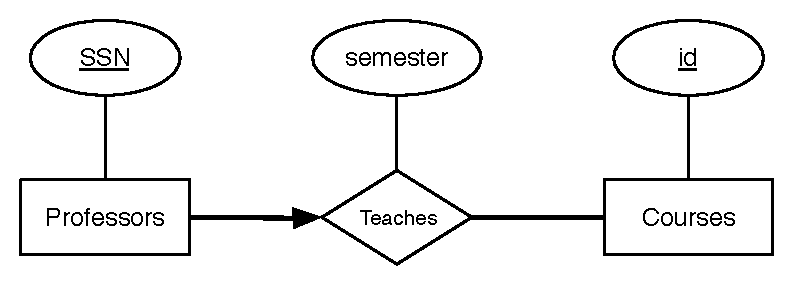
\includegraphics[scale=.5]{2_2_5.eps}
      } \qquad
      \subfigure[ER Diagram for 2.2-6]{
        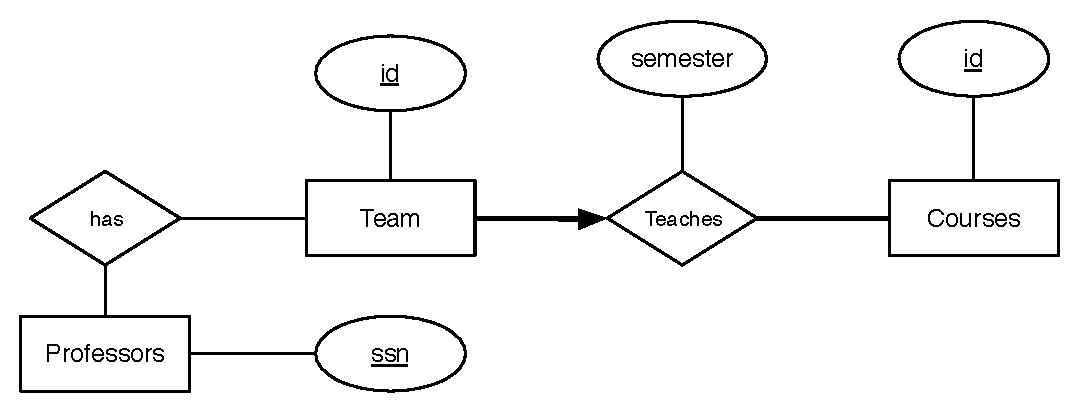
\includegraphics[scale=.5]{2_2_6.eps}
      } \qquad
    \end{figure}
  \end{solution}
\end{problem}

\begin{problem}{2.4}

  A company database needs to store information about employees (identified by ssn, with salary and phone as
  attributes), departments (identified by dna, with dname and budget as attributes), and children of employees (with
  name and age as attributes). Employees work in departments; each department is managed by an employee; a child must be
  identified uniquely by name when the parent (who is an employee; assume that only one parent works for the company) is
  known. We are not interested in information about a child once the parent leaves the company. \\

  \noindent Draw an ER diagram that captures this information.

  \begin{solution}
    \begin{figure}[H]
      \centering
      \caption{ER Diagram}
      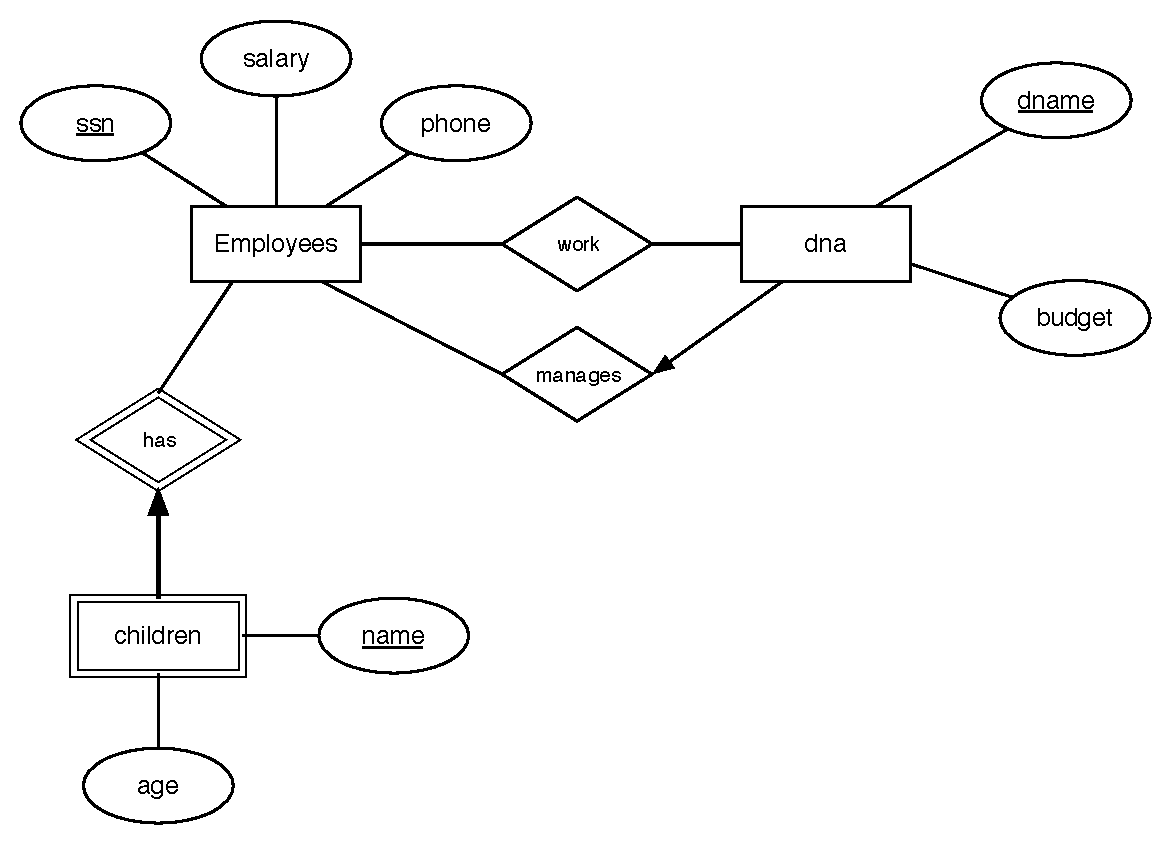
\includegraphics[scale=.5]{2_4.eps}
    \end{figure}
  \end{solution}
\end{problem}

\begin{problem}{2.6 (1)}

  Computer Sciences Department frequent fliers have been complaining to Dane County Airport officials about the poor
  organization at the airport. As a result, the officials decided that all information related to the airport should be
  organized using a DBMS, and you have been hired to design the database. Your first task is to organize the information
  about all the airplanes stationed and maintained at the airport. The relevant information is as follows:

  \begin{itemize}
    \item Every airplane has a registration number, and each airplane is of a specific model.
    \item The airport accommodates a number of airplane models, and each model is identified by
          a model number (e.g., DC-lO) and has a capacity and a weight.
    \item A number of technicians work at the airport. You need to store the name, SSN, address,
          phone number, and salary of each technician.
    \item Each technician is an expert on one or more plane model(s), and his or her expertise may overlap with that of other technicians.      This information about technicians must also be recorded.
    \item Traffic controllers must have an annual medical examination. For each traffic controller, you must store the
          date of the most   recent exam.
    \item All airport employees (including technicians) belong to a union. You must store the union membership number of
          each employee. You can assume that each employee is uniquely identified by a social security number.
    \item The airport has a number of tests that are used periodically to ensure that airplanes are still airworthy.
          Each test has a Federal Aviation Administration (FAA) test number, a name, and a maximum possible score.
    \item The FAA requires the airport to keep track of each time a given airplane is tested by a given technician using
          a given test. For each testing event, the information needed is the date, the number of hours the technician
          spent doing the test, and the score the airplane received on the test.
  \end{itemize}

  \noindent Draw an ER diagram for the airport database. Be sure to indicate the various attributes of each entity and
  relationship set; also specify the key and participation constraints for each relationship set. Specify any necessary
  overlap and covering constraints a.s well (in English).

  \begin{solution}
    \begin{figure}[H]
      \centering
      \caption { ER Diagram }
      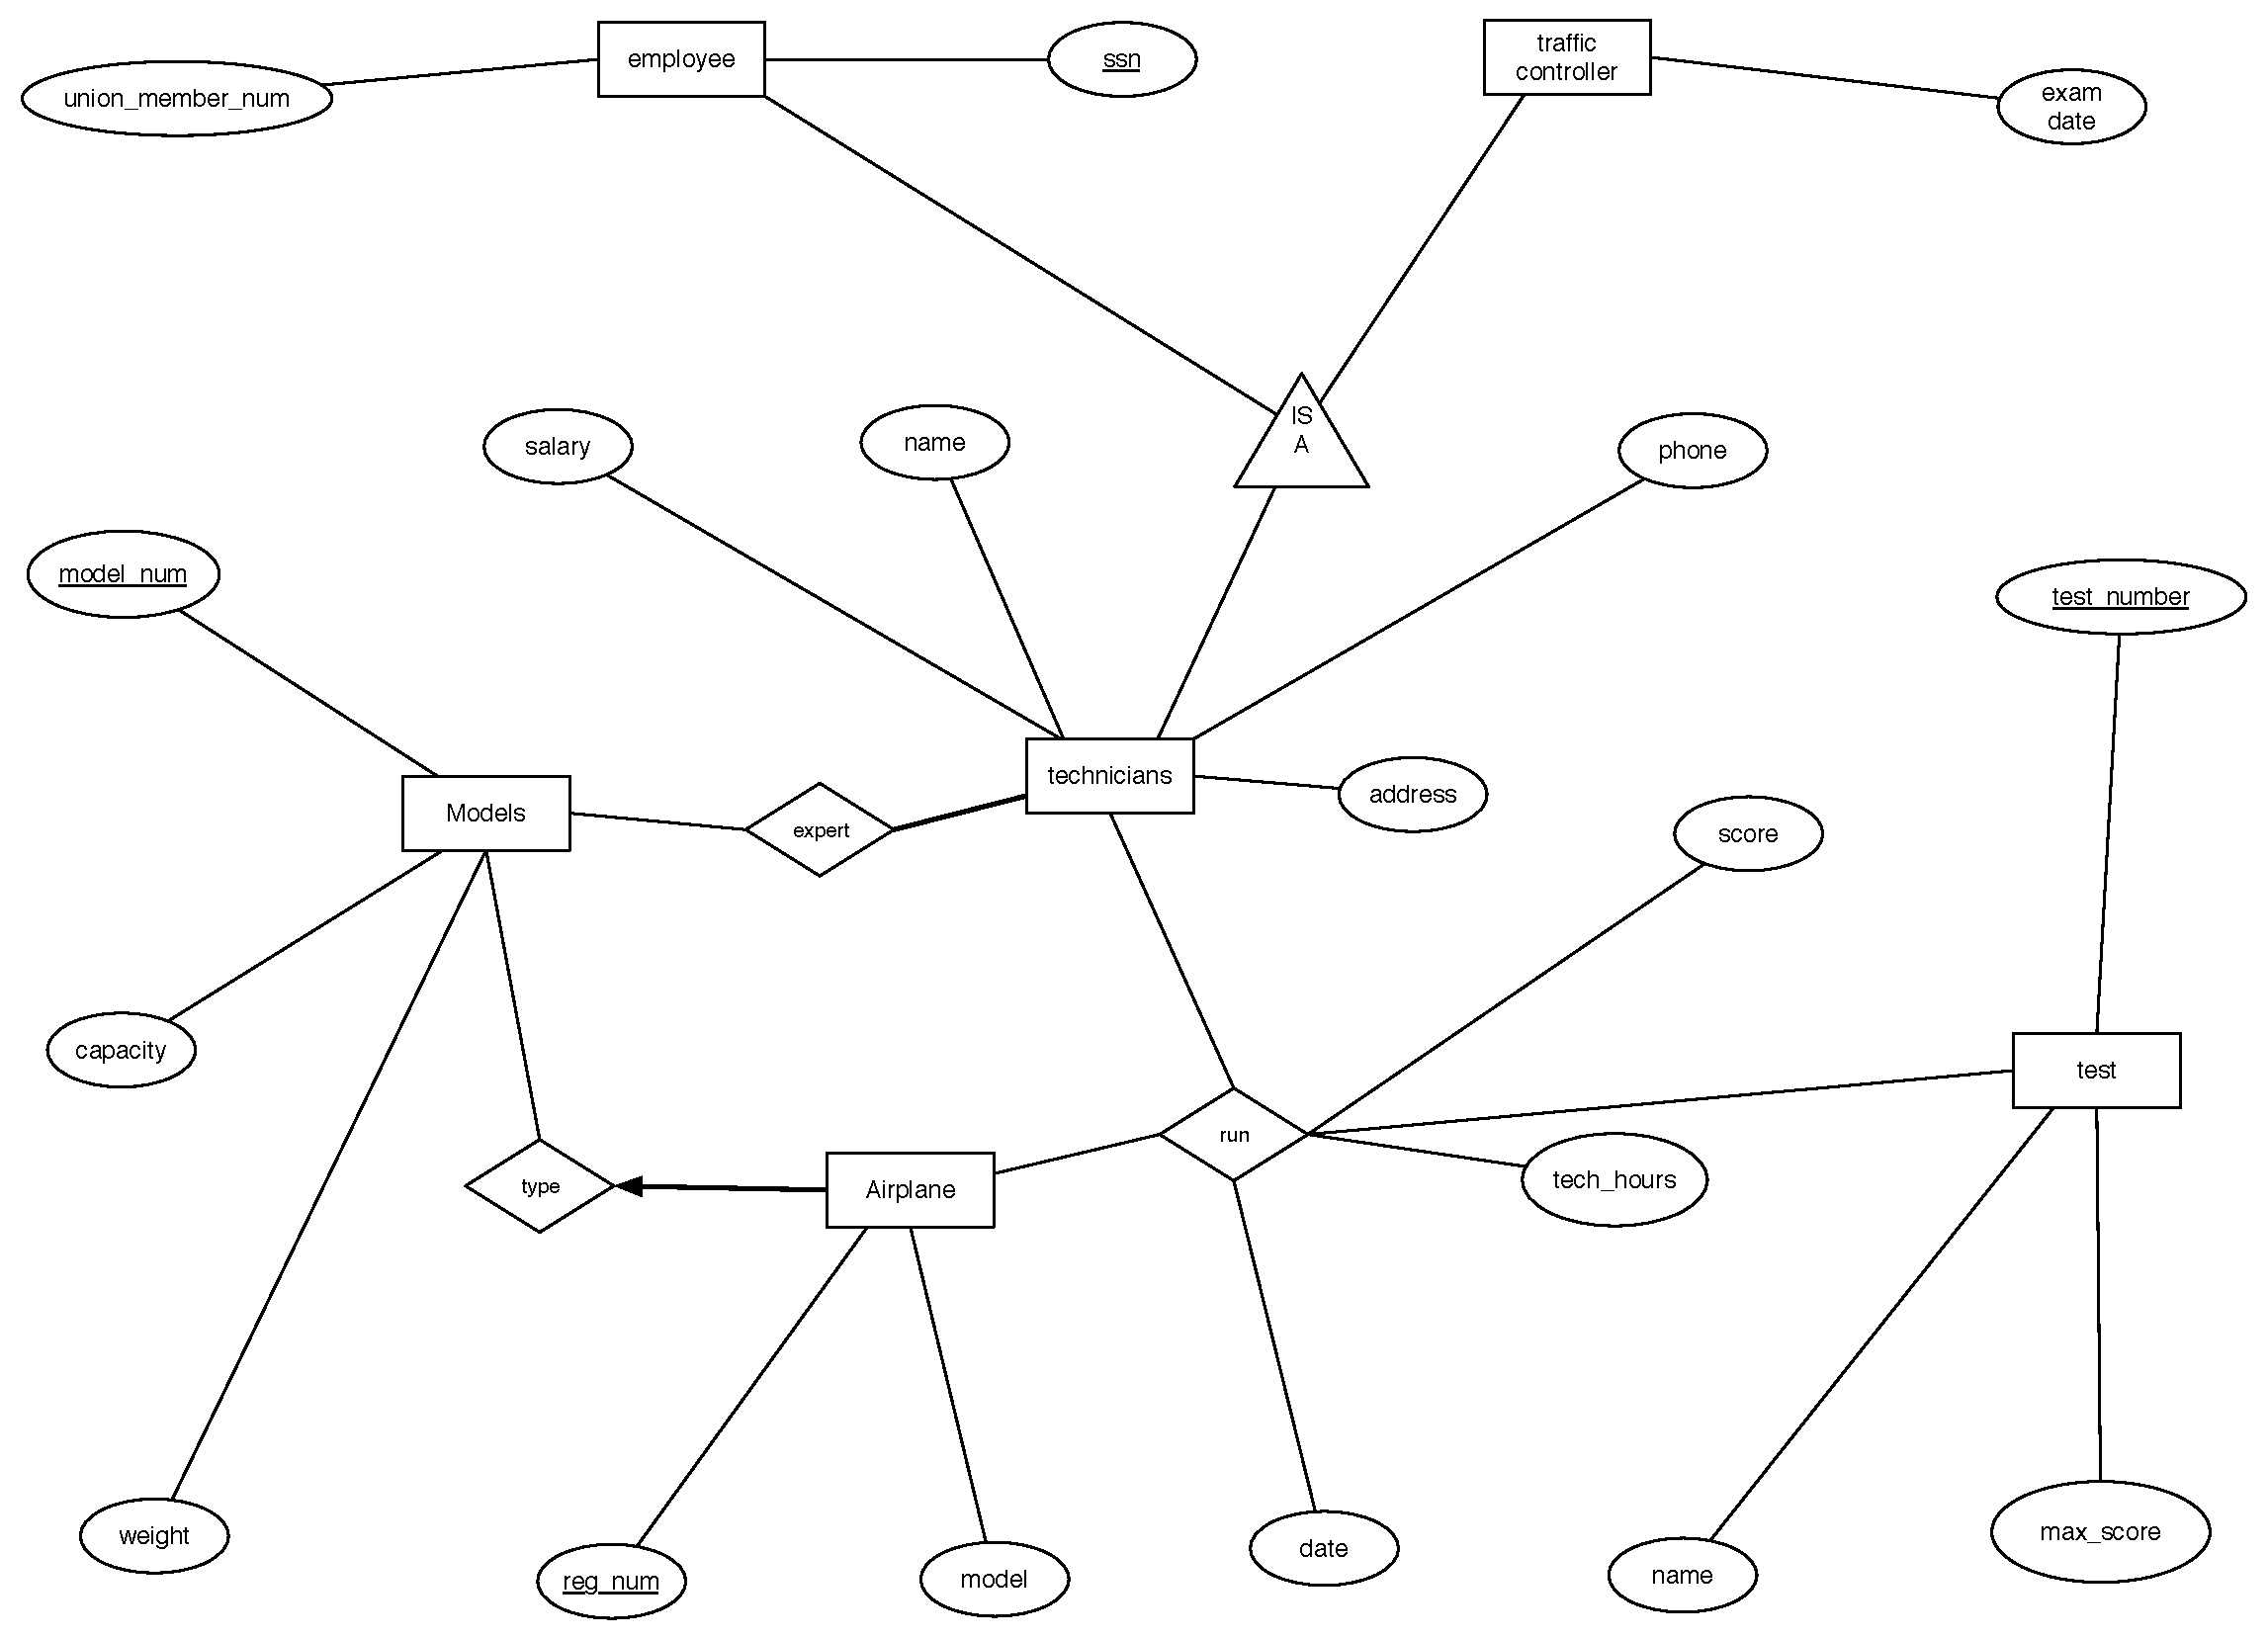
\includegraphics[scale=.4]{2_6.eps}
    \end{figure}
  \end{solution}
\end{problem}

\begin{problem}{2.8}

  Although you always wanted to be an artist, you ended up being an expert on databases because you love to cook data
  and you somehow confused database with data baste. Your old love is still there, however, so you set up a database
  company, ArtBase, that builds a product for art galleries. The core of this product is a database with a schema that
  captures all the information that galleries need to maintain. Galleries keep information about artists, their names
  (which are unique), birthplaces, age, and style of art. For each piece of artwork, the artist, the year it was made,
  its unique title, its type of art (e.g., painting, lithograph, sculpture, photograph), and its price must be stored.
  Pieces of artwork are also classified into groups of various kinds, for example, portraits, still lifes, works by
  Picasso, or works of the 19th century; a given piece may belong to more than one group. Each group is identified by a
  name (like those just given) that describes the group. Finally, galleries keep information about customers. For each
  customer, galleries keep that person's unique name, address, total amount of dollars spent in the gallery (very
  important!), and the artists and groups of art that the customer tends to like. \\

  \noindent Draw the ER diagram for the database.

  \begin{solution}
    \begin{figure}[H]
      \centering
      \caption { ER Diagram }
      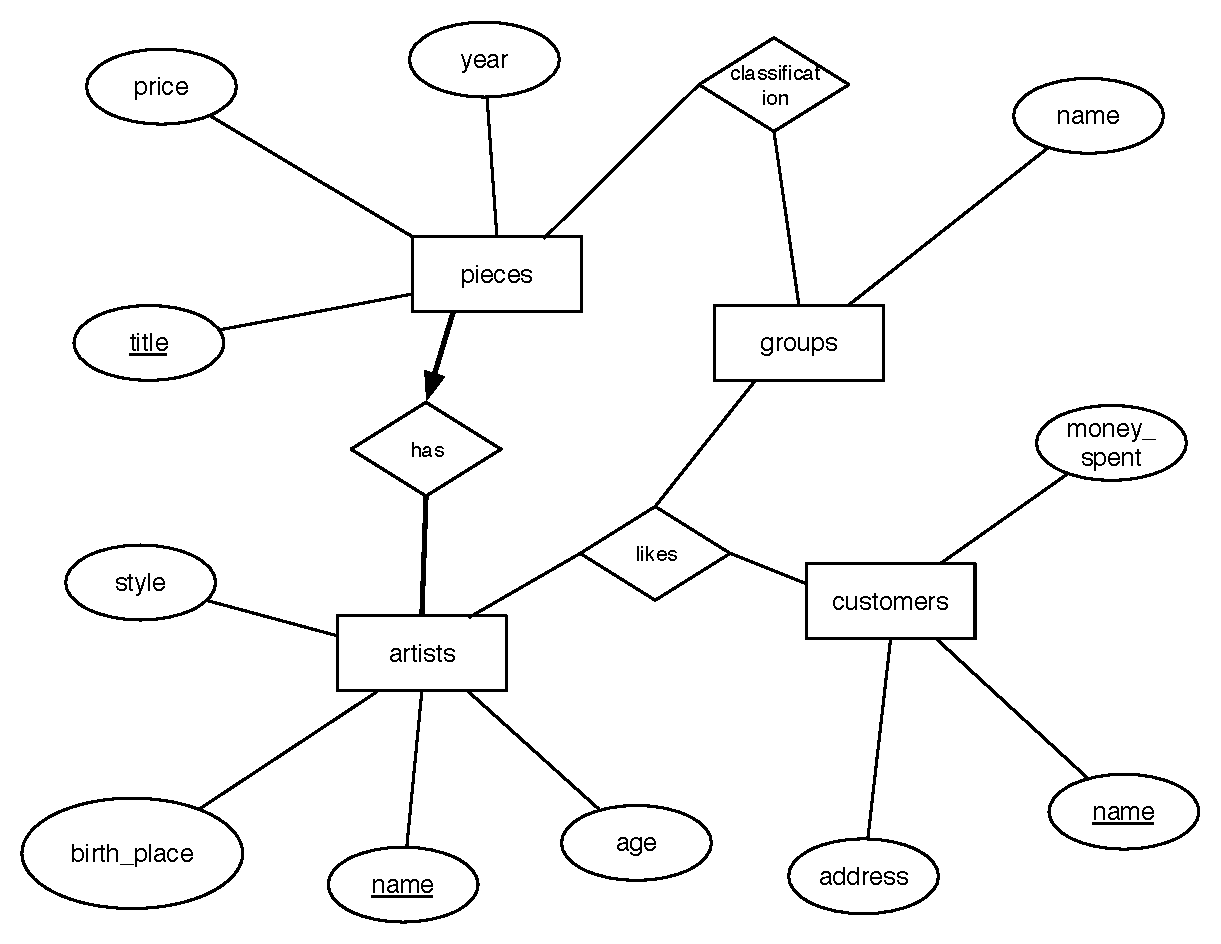
\includegraphics[scale=.5]{2_8.eps}
    \end{figure}
  \end{solution}
\end{problem}


\end{document}
